\documentclass[12pt]{article}

\usepackage[left=1in,top=1in,right=1in,bottom=1in]{geometry}
\usepackage{graphicx} % Required for the inclusion of images
\graphicspath{{../img/proposal/}}
\usepackage{float}
\usepackage{comment}
\usepackage{titlesec}
\setlength\parindent{24pt} %space for indentation
%\font\regfont=cmr12 at 13pt

% The title of your proposal should be informative, and must not exceed two printed lines. Please use mixed case instead of all upper case.
\title{\Large \textbf{Correcting Keck/NIRC2's Systematic Errors \\ Using Linear SVMs}}
\author{Justin Kang}
\date{\today}

\begin{document}
\thispagestyle{empty}
\maketitle


\thispagestyle{empty}
\section*{Abstract}
% Write a concise abstract describing the proposed investigation, including the main science goals and the justification for requesting observations or funding from HST. The abstract must be written in standard ASCII and should be no longer than 20 lines of 85 characters of text. This limit is enforced by APT.
\noindent Keck/NIRC2 uses AO to produce the highest-resolution ground-based images and spectroscopy in the 1-5 micrometer range. It is one of the best instruments for planet discovery and characterization, with 44 papers published just this year that have used it. However, there are several systematic errors that reduce its effectiveness and usability. Examples of these are read errors mirrored across the image quadrants, and the noisier lower-left quadrant. The current method of dealing with this noise is using a three-point dither pattern to reduce the effects of the bad quadrant, and there is no real method of dealing with the mirrored errors as of yet.\\\\ 
We propose to instead create a model of these errors. By doing so, we can then attempt to eliminate the bad quadrant, allowing for more usable image space, and also improve the deepness of the images by removing instrumental noise in all quadrants. One possiblity is training a linear support vector machine and using it to classify sources as either real or noise. Linear classifiers are compact, fast to train, fast to execute, and can be trained on large amounts of data, making them an ideal tool for this application. Furthermore the KOA database makes readily available large amounts of both training and testing data. Thus by successfully modeling and eliminating this noise, we can improve one of the best ground-based instruments for future use.


\newpage
\setcounter{page}{1}
\section*{Scientific Justification}
% This section should present a balanced discussion of background information, the program’s goals, its significance to astronomy in general, and its importance for the specific sub-field of astronomy it addresses. 
% AR Proposals should describe how the project improves upon or adds to the previous use of the data.
% Calibration Proposals should describe what science will be enabled by the successful completion of the program, and how the currently supported core capabilities, their calibrations, and the existing pipeline or data reduction software are insufficient to meet the requirements of this type of science.
\subsection*{Direct Imaging}
% https://en.wikipedia.org/wiki/Methods_of_detecting_exoplanets#Direct_imaging
Direct imaging for planet detection, as the name suggests, involves directly taking images of a planetary system (or debris disk). From a series of images, we can estimate the planet's orbit, size, temperature, atmosphere, and other properties from its photometry, colors, and spectra. This method favors planets that can be resolved from the host star(s) - thus young and hot planets that are still radiating away energy from their creation (primordial thermal emission), widely separated from their host, and large (several times that of Jupiter). Unlike most other detection methods, direct imaging works best with face-on orbits rather than edge-on, as it can then accurately measure the entirety of the planet's orbit around the star. This gives direct imaging a unique parameter space in relation to the other detection methods - it finds large planets with large orbital radii, occupying the space beyond what current radial velocity methods detect. Thus the method complements well the other detection methods, such as radial velocity and transits.\\

\subsection*{Keck/NIRC2}
% https://en.wikipedia.org/wiki/W._M._Keck_Observatory#Instruments
% https://www2.keck.hawaii.edu/inst/nirc2/
% https://www2.keck.hawaii.edu/inst/nirc2/ObserversManual.html
The second generation Near-Infrared Camera (NIRC2) at Keck Observatory uses the Keck Adaptive Optics system to produce the current highest-resolution ground-based images and spectroscopy in the 1-5 micrometer range. Its first major planet discovery was in Marois et al. (2008), where it was use to observe the first multiplanet system in HR 8799. Since then it has been widely used by the direct imaging community, with 44 papers published in just 2017 that used the instrument.\\
\indent \textbf{However, there are several systematic errors that reduce NIRC2's effectiveness and usability}. The first example of these is the lower-left quadrant of the array; as noted by many that have used it (Bowler et al. (2014), Crossfield et al. (2017), Rodriguez et al. (2017)), this corner suffers from elevated noise levels. This noise presents itself in the form of vertical stripes - here we see groups of 8 vertical pixels with increased intensity, repeated in a stripe pattern across the entire quadrant. The current popular method of dealing with this quadrant is adopting a 3-point dither pattern (as suggested in the Keck observer's manual), which omits the lower left and central positions of the detector. Another method is to place the coronagraph far from the region, keeping the objects of interest outside the region. Both of these "solutions" avoid the use of the error-prone region, losing an entire quadrant of the detector. Thus, these aren't really useful or efficient methods - we need a better way of dealing with this error. There is another similar systematic error - across images we can see groups of eight horizontal pixels with increased intensity, mirrored across each of the quadrants. A consequence of detection in the near-infrared, this error is also commonly handled in a similar way - by not actually systematically dealing with the error itself, but raising the criteria for detections of real objects such that this error is below a threshold and ignored. Thus these solutions for NIRC2's systematic errors leave a lot to be desired, and call for better techniques to deal with them.

\subsection*{Linear SVMs and the Sliding Window Detection}
% https://en.wikipedia.org/wiki/Support_vector_machine
We now introduce a technique commonly used in the field of computer vision - the sliding window classification from Dalal and Triggs (2005), used commonly in pedestrian detection. This algorithm employs a sliding window to independently classify all iimage windows as being an object or non-object. Given heterogeneous training and testing data, we transform images to a histogram-of-gradients representation, train a linear classifier, and use this classifier to classify up to millions of sliding windows. Here the training data is initially a combination of positive training examples and a negative set free of the sample. The classifier is then trained, and the negative examples are searched for false positives. The classifier is then retrained using the initial set and the false positives to improve accuracy.\\
\indent The benefits of using linear classifiers are that they are compact, fast to train, and fast to execute, allowing for quick verification of the results. The one we use here is a support vector machine - given a set of training examples, which are annotated as belonging to one of two categories (e.g. object or non-object), SVMs build a model that assigns new examples to one of the categories. The model is a representation of the examples as points in spaced, mapped so that the examples of the separate categories are divided by the widest gap possible. New examples are then mapped to that same space, and are assigned a category based on which side of the gap they're on. 

\subsection*{Proposed Program}
% This section should present a balanced discussion of background information, the program’s goals, its significance to astronomy in general, and its importance for the specific sub-field of astronomy it addresses. 
% AR Proposals should describe how the project improves upon or adds to the previous use of the data.
% Calibration Proposals should describe what science will be enabled by the successful completion of the program, and how the currently supported core capabilities, their calibrations, and the existing pipeline or data reduction software are insufficient to meet the requirements of this type of science.


\newpage
\begin{figure}[H]
\centering
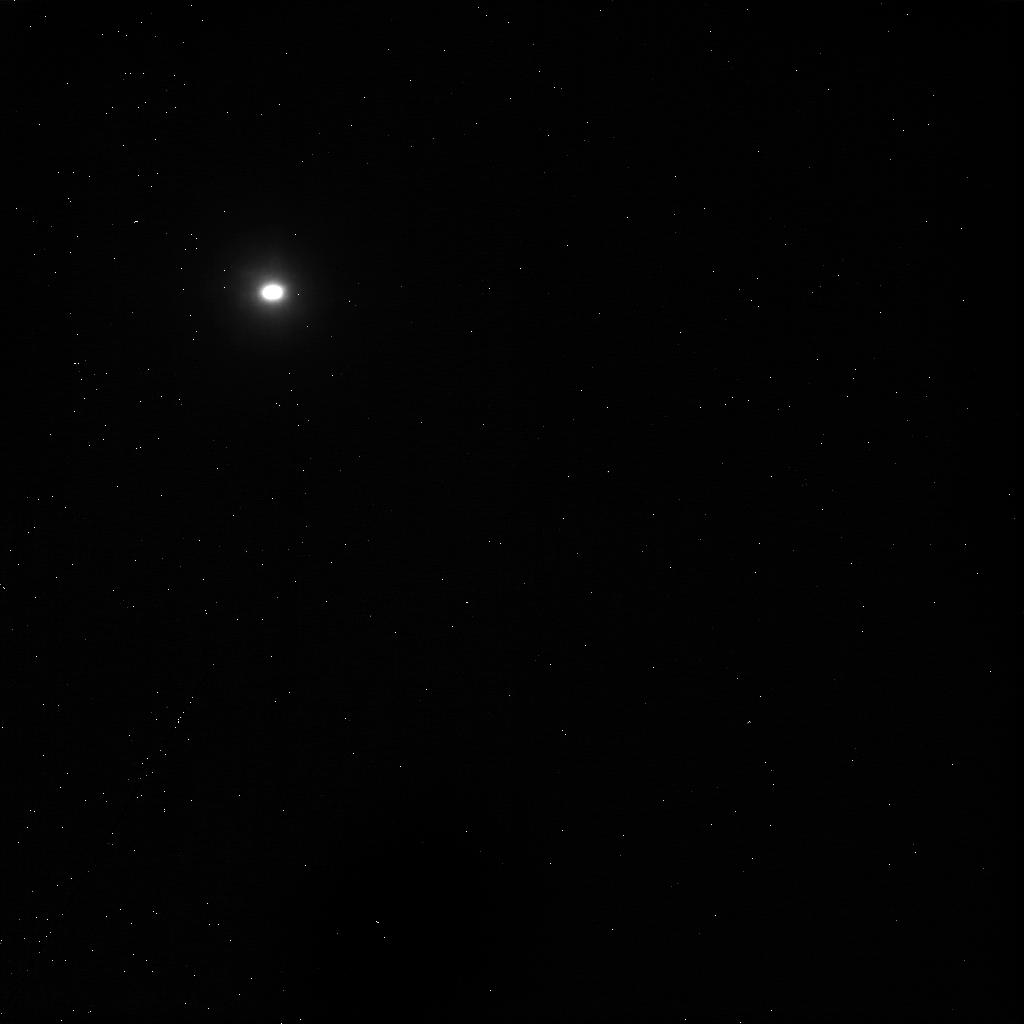
\includegraphics[width=0.45\textwidth]{dither1.jpg}
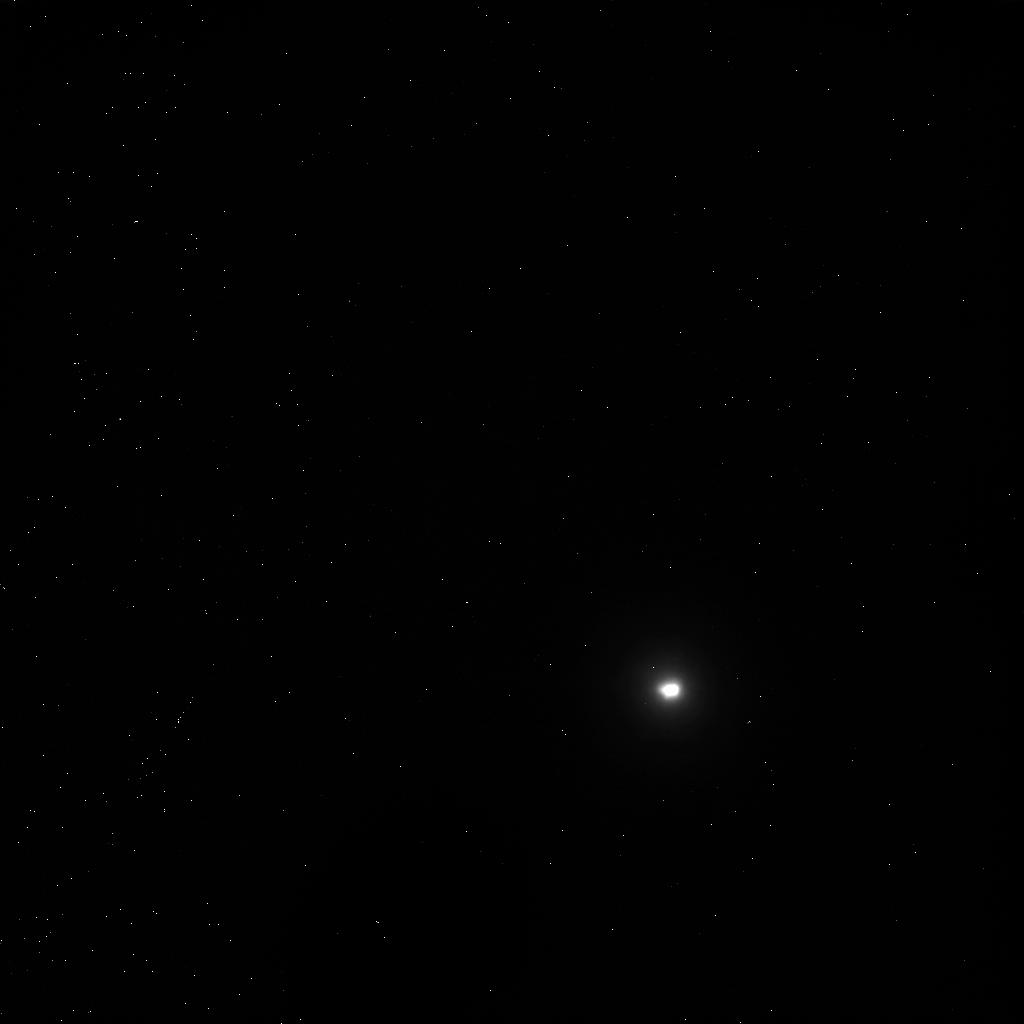
\includegraphics[width=0.45\textwidth]{dither2.jpg}
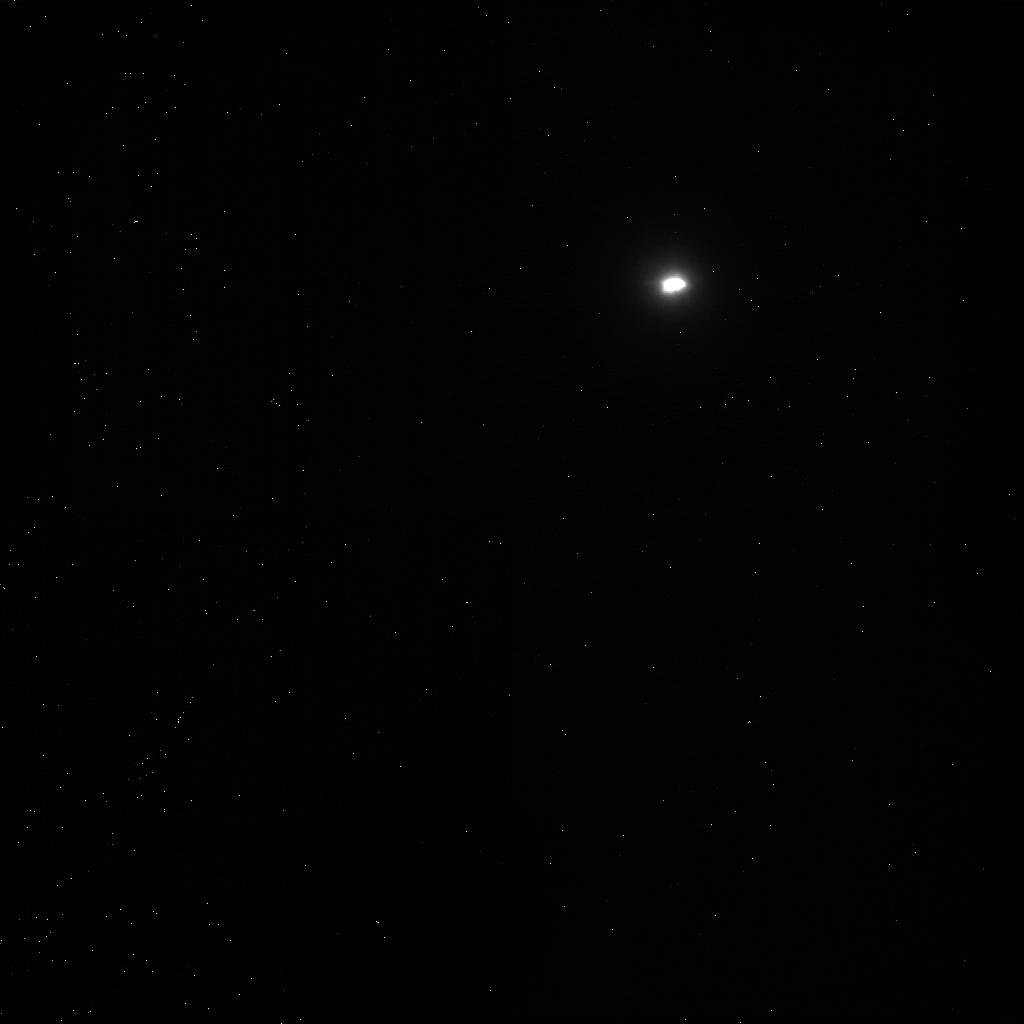
\includegraphics[width=0.45\textwidth]{dither3.jpg}
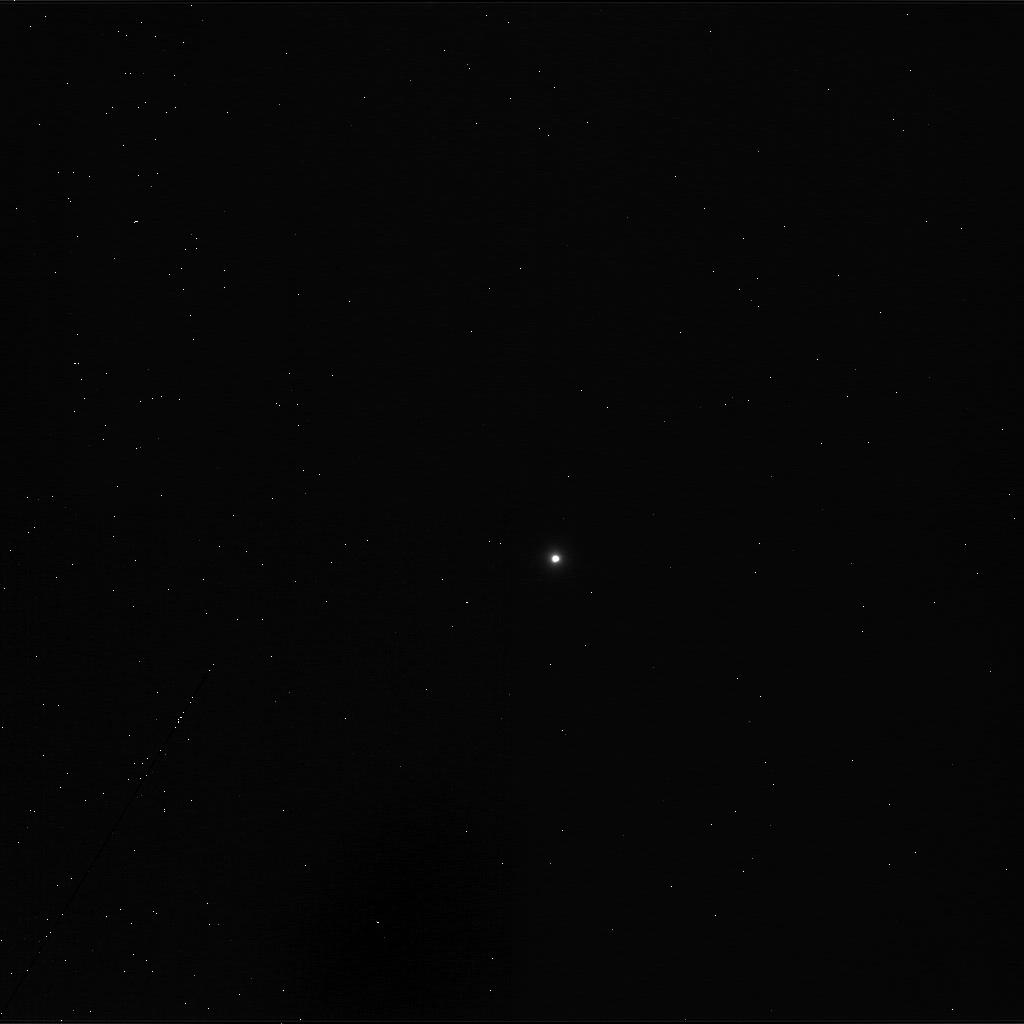
\includegraphics[width=0.45\textwidth]{dither4.jpg}
\caption{From Kraus et al. (2006), a very low mass star in the substellar boundary in Taurus. Here we see a 4-point dither pattern, which literature suggests has an improvement in the signal-to-noise over simpler dither patterns.}
\end{figure}
\begin{figure}[H]
\centering
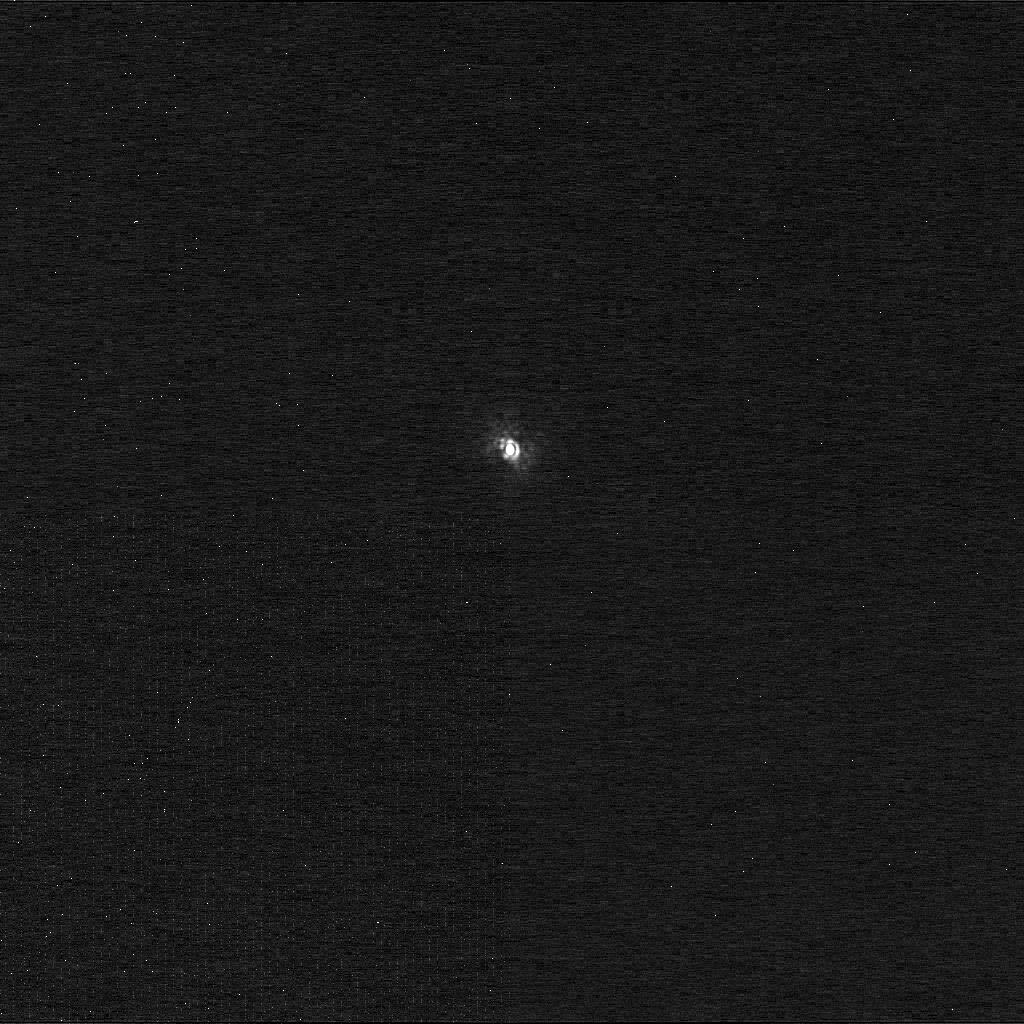
\includegraphics[width=0.45\textwidth]{image.jpg}

\includegraphics[width=0.45\textwidth]{corner.jpg}
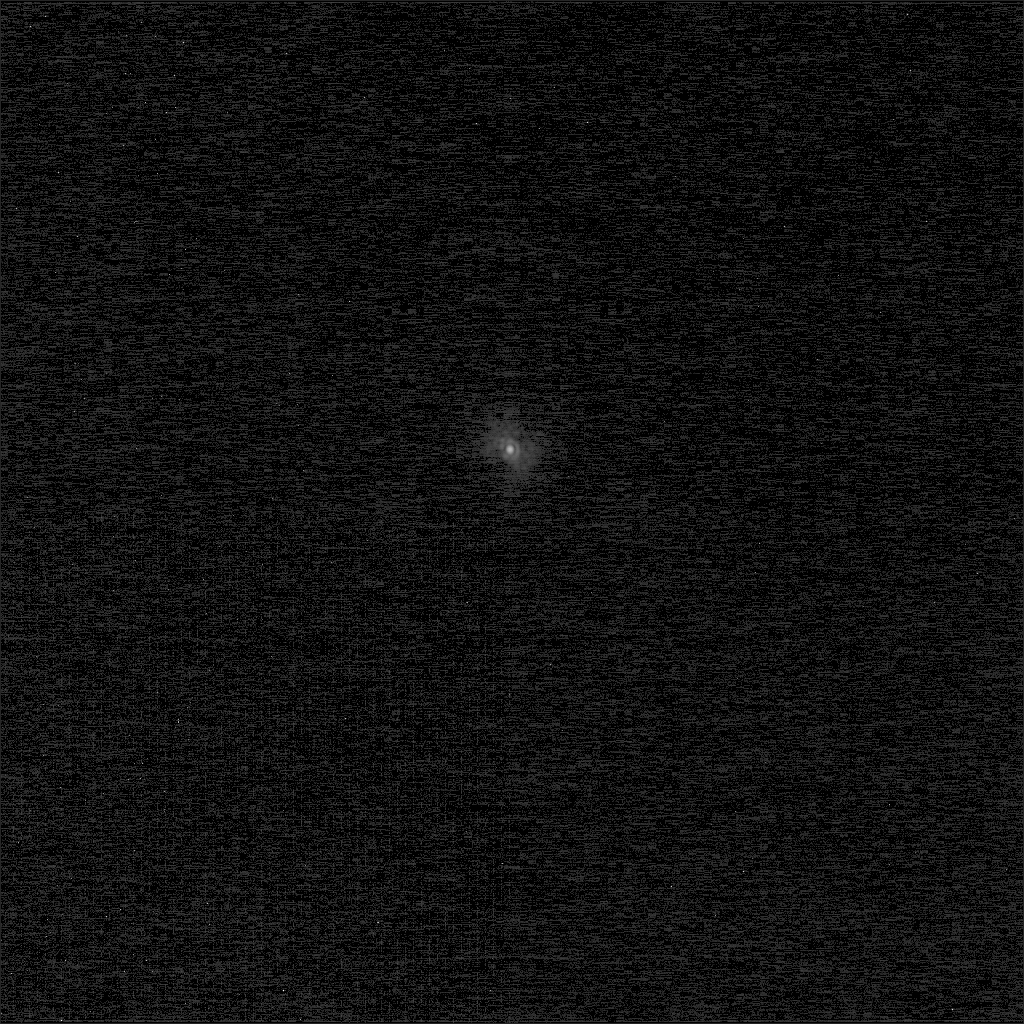
\includegraphics[width=0.45\textwidth]{image_root.png}

\includegraphics[width=0.45\textwidth]{corner_root.png}
\caption{From Bryan et al. (2016), ROXs 12 and its planetary companion. The left column shows the full image from Keck/NIRC2, while the right column shows a zoom-in of the lower-left quadrant. The images on the bottom row show the fourth root of the intensities of the image, to better demonstrate the enhanced noise seen in that quadrant.}
\end{figure}


\newpage
\section*{Analysis Plan}
% All AR Proposals should provide a detailed data analysis plan and describe the datasets that will be analyzed. Proposers should complete the information required in the APT dataset table (see Section 8.14): the number of datasets (not pointings) per instrument needed to carry out the research and the type of data retrieval (ftp, DVD, or disk: see the HST Archive Data Retrieval Options for a description of the available options). Proposers must provide a schedule indicating the timescale for the data request(s), for example all datasets at once, or 1/12th of the datasets per month. Inclusion of a complete target list is not required.
% Calibration Proposals should discuss what documentation, and data products and/or software will be made available to STScI to support future observing programs. Proposers should explain how their programs complement ongoing calibration efforts by the instrument groups. They should contact the relevant groups to ensure that efforts are not duplicated.
blah blah blah


\newpage
\section*{Management Plan}
% Provide a concise, but complete, management plan. This plan will be used by the review panels to assess the likely scale of the proposed research program. Proposers should include a schedule of the work required to achieve the scientific goals of the program, a description of the roles of the PI, Co-Is, postdocs, and students who will perform the analysis, and a plan to disseminate the results to the community.
blah blah blah


\newpage
\section*{References}
\bibliography{mybib}

% https://arxiv.org/pdf/0811.2606.pdf
% https://arxiv.org/pdf/1411.3722.pdf
% http://iopscience.iop.org/article/10.3847/1538-3881/aa6e01
% https://arxiv.org/pdf/1709.01957.pdf
% http://www.csd.uwo.ca/~olga/Courses/Fall2009/9840/Papers/DalalTriggsCVPR05.pdf
% https://arxiv.org/pdf/astro-ph/0602449.pdf
% https://arxiv.org/pdf/1606.06744.pdf

\end{document}